\documentclass[conference]{IEEEtran}
\usepackage{cite}
\usepackage{amsmath,amssymb,amsfonts}
\usepackage{algorithmic}
\usepackage{graphicx}
\usepackage{textcomp}
\usepackage{xcolor}
\usepackage{hyperref}
\usepackage{booktabs}
\usepackage{array}
\usepackage{tikz}
\usetikzlibrary{shapes,arrows.meta,positioning,fit,backgrounds,shapes.geometric,calc}

\hypersetup{colorlinks=false, pdfborder={0 0 0}}

\tikzset{
  layer/.style={draw=black!70, thick, rounded corners=4pt, dashed, fill=gray!5},
  blk/.style={rectangle, draw=black!80, fill=#1, rounded corners=2pt,
              minimum height=0.6cm, text centered, font=\footnotesize, inner sep=4pt},
  blk/.default=blue!12,
  dblk/.style={cylinder, shape border rotate=90, draw=black!80, fill=red!15,
               minimum height=0.9cm, minimum width=1.5cm, font=\footnotesize,
               text centered, shape aspect=0.35},
  cblk/.style={rectangle, draw=black!80, fill=green!15, rounded corners=6pt,
               minimum height=0.7cm, text centered, font=\footnotesize, inner sep=4pt},
  arr/.style={-{Stealth[length=4pt,width=3pt]}, thick},
  darr/.style={{Stealth[length=4pt,width=3pt]}-{Stealth[length=4pt,width=3pt]}, thick},
}

\begin{document}

\title{AI-Powered Multi-Lingual News Aggregation and Exam-Focused Summarization System for Competitive Examination Preparation}

\author{
  \IEEEauthorblockN{Arshi Shaikh}
  \IEEEauthorblockA{\textit{Dept. of Computer Engineering}\\
    \textit{M.H. Saboo Siddik Polytechnic}\\
    Byculla, Mumbai\\
    arshishaikh9214@gmail.com}
  \and
  \IEEEauthorblockN{Arshiya Shirgaonkar}
  \IEEEauthorblockA{\textit{Dept. of Computer Engineering}\\
    \textit{M.H. Saboo Siddik Polytechnic}\\
    Byculla, Mumbai\\
    arshiyashirgaonkar2007@gmail.com}
  \and
  \IEEEauthorblockN{Ayesha Shaikh}
  \IEEEauthorblockA{\textit{Dept. of Computer Engineering}\\
    \textit{M.H. Saboo Siddik Polytechnic}\\
    Byculla, Mumbai\\
    engrayesha2008@gmail.com}
  \and
  \IEEEauthorblockN{Prof. Mohammad Ali (Guide)}
  \IEEEauthorblockA{\textit{Dept. of Computer Engineering}\\
    \textit{M.H. Saboo Siddik Polytechnic}\\
    Byculla, Mumbai}
}

\maketitle

\begin{abstract}
Competitive examination candidates in India face significant challenges aggregating relevant current affairs across multiple years while efficiently analyzing educational documents. This paper presents a novel AI-powered system addressing these challenges through three key innovations: (1)~a hybrid RSS-archive aggregation engine retrieving news articles spanning a decade from 10+ Indian sources; (2)~an exam-focused PDF and text analysis module utilizing Groq's Llama~3.3~70B model to extract examination-relevant insights; and (3)~a multi-lingual processing pipeline supporting 11 Indian languages with native script rendering. The system employs a three-tier architecture comprising a React-TypeScript frontend, Express.js backend, and SQLite database with Write-Ahead Logging, achieving 150\,ms average API response time and supporting documents up to 50\,MB. System testing demonstrates 87\% relevance accuracy in content extraction and 3.2\,s average processing time for comprehensive document analysis. The system uniquely combines temporal news aggregation, AI-driven exam relevance scoring, and cross-device synchronization, providing a targeted solution for Indian competitive examination preparation.
\end{abstract}

\begin{IEEEkeywords}
News Aggregation, Natural Language Processing, Competitive Examinations, Multi-lingual AI, Document Analysis, Educational Technology, Large Language Models
\end{IEEEkeywords}

%==========================================================
\section{Introduction}
%==========================================================

Competitive examinations in India—including UPSC Civil Services, SSC, Banking, and State Public Service Commissions—require candidates to maintain comprehensive knowledge of current affairs spanning multiple years. Traditional news consumption methods present three critical challenges: (1)~\textit{temporal fragmentation}, where relevant news is scattered across years without centralized access; (2)~\textit{content overload}, where candidates cannot efficiently identify examination-relevant information from the daily news deluge; and (3)~\textit{linguistic barriers}, which restrict access to vernacular content for regional language candidates.

Existing news aggregation platforms such as Google News, Inshorts, and Dailyhunt focus on real-time delivery but lack historical depth, exam-specific analysis, and comprehensive multi-lingual support. Academic research in text summarization~\cite{allahyari2017text, alomari2022deep} primarily addresses generic summarization without domain-specific optimization for educational contexts. No existing system simultaneously offers decade-spanning news retrieval, AI-powered exam relevance extraction, and unified multi-format document analysis.

This paper introduces a comprehensive system with three novel contributions:

\textbf{Temporal News Aggregation Engine:} A hybrid architecture combining RSS feed processing for recent content ($\leq$7 days) and date-parameterized web scraping for historical archives (up to 10 years). The system aggregates from Times of India, The Hindu, Indian Express, NDTV, Hindustan Times, and six additional sources, processing 1{,}000+ articles daily across nine syllabus-aligned topic categories.

\textbf{Exam-Focused AI Analysis:} Domain-specific prompting with Groq's Llama~3.3~70B Versatile model extracts examination-relevant insights including factual key takeaways (names, dates, numbers), potential examination questions, topic interconnections, and syllabus relevance scores. The pipeline processes news articles and uploaded PDF documents with identical analytical rigor via a four-stage error-recovery JSON parser.

\textbf{Multi-Lingual Processing Pipeline:} Native support for 11 Indian languages (English, Hindi, Tamil, Bengali, Telugu, Marathi, Gujarati, Kannada, Malayalam, Punjabi, Urdu) with Unicode script rendering. Native-script output is enforced via explicit LLM prompting, eliminating transliteration artifacts that degrade comprehension for regional candidates.

The architecture implements JWT-based authentication, cross-device synchronization via RESTful APIs, and SQLite with Write-Ahead Logging. System benchmarks report 150\,ms average API response, 3.2\,s document analysis, and 87\% exam relevance accuracy.

%==========================================================
\section{Related Work}
%==========================================================

\subsection{Text Summarization Techniques}
Allahyari et al.~\cite{allahyari2017text} comprehensively survey extractive and abstractive summarization, covering statistical features, graph-based methods (TextRank), and lexical chains~\cite{alam2003structured}. While effective for general use, these approaches lack semantic understanding and domain adaptation. Deep learning advances~\cite{alomari2022deep} yield transformer-based systems (BERT, GPT, T5), but factual hallucination remains a concern for exam preparation~\cite{cao2022hallucinated}. Our system mitigates this through explicit fact-extraction prompting, structured JSON output, and source attribution.

\subsection{Multi-Lingual NLP Systems}
Aharoni et al.~\cite{aharoni2022mface} introduce mFACE for multilingual summarization with factual consistency evaluation, focusing on high-resource European languages. Indian languages present distinct challenges in tokenization, script rendering, and morphological diversity. Our approach uses native LLM processing with language-specific system prompts, falling back to Google Translate API only for cross-lingual access—preserving linguistic authenticity over aggressive translation.

\subsection{News Aggregation Systems}
Commercial aggregators such as Google News employ collaborative filtering but provide no temporal depth beyond 30 days and no domain-specific analysis. Amato et al.~\cite{amato2017semantic} propose semantic summarization of heterogeneous news, focusing solely on real-time feeds. Our hybrid RSS-archive approach is, to our knowledge, the first documented system combining live feed aggregation with date-parameterized historical scraping across a decade of Indian news archives.

\subsection{Educational Technology Systems}
Educational chatbots and LMS platforms provide structured content delivery but lack current affairs integration. Alias~\cite{alias2021unsupervised} demonstrates value in domain-specific feature extraction for academic chatbots using constrained FP-growth. Our work extends this concept by employing LLM-based extraction with examination syllabus awareness and unified processing of heterogeneous document formats.

\textbf{Research Gap:} No existing system combines (1)~decade-spanning news aggregation, (2)~exam-specific AI analysis with factual accuracy safeguards, (3)~comprehensive Indian language support with native-script enforcement, and (4)~unified processing of news and educational documents. This work addresses that gap with a functional, deployed prototype.

%==========================================================
\section{Methodology}
%==========================================================

\subsection{System Requirements and Design Principles}
Requirements were identified through a review of UPSC, SSC, and Banking examination syllabi and informal discussions with students in the authors' institution:

\begin{itemize}[leftmargin=*, nosep]
  \item \textbf{R1 – Temporal Coverage:} Access to news articles from the past decade to support multi-year preparation cycles.
  \item \textbf{R2 – Exam Relevance:} Automatic extraction of syllabus-aligned facts, eliminating irrelevant content.
  \item \textbf{R3 – Multi-Format Processing:} Unified analysis of news articles, PDFs, and pasted text.
  \item \textbf{R4 – Linguistic Accessibility:} Native script support for regional candidates without transliteration.
\end{itemize}

Design principles: (1)~modular architecture for independent scaling; (2)~API-first design enabling cross-device synchronization; (3)~progressive enhancement with graceful API fallbacks; (4)~per-user data isolation via JWT.

\subsection{Hybrid News Aggregation Architecture}
The aggregation engine uses a dual-mode strategy:

\textbf{RSS Mode ($\leq$7 days):} Fetches RSS feeds from 10+ Indian sources, parsing title, description, publication timestamp, and URL. CORS proxy handling manages cross-origin constraints. Deduplication applies Levenshtein distance (threshold 0.85) to eliminate near-duplicate headlines across sources.

\textbf{Archive Mode ($>$7 days):} Date-parameterized URL construction accesses newspaper archive endpoints (e.g., \texttt{timesofindia.com/archive/YYYY/MM/DD}). DOM-specific parsers extract article links and full content. Rate limiting (3\,s inter-request delay) prevents server overload; exponential backoff handles transient failures. A 30-day range retrieves 400–500 deduplicated articles.

Topic classification uses keyword matching against nine predefined dictionaries aligned to UPSC/SSC syllabus categories (Economy, Polity, Environment, International Relations, Science \& Technology, Society, History, Geography, General). Multi-label assignment is supported.

\subsection{AI-Powered Exam-Focused Analysis Pipeline}
Content is processed in four stages:

\textbf{Stage 1 – Content Extraction:} Full-text scraping retrieves complete article content beyond RSS snippets. PDF.js~(v4.9.155) extracts text from all pages of documents up to 50\,MB. Pasted text bypasses extraction.

\textbf{Stage 2 – Preprocessing:} HTML entity removal, whitespace normalization, and truncation to 6{,}000 characters for LLM context optimization. Language detection tags content for routing.

\textbf{Stage 3 – LLM Analysis:} Groq's \texttt{llama-3.3-70b-versatile} model is invoked with an exam-specific system prompt requiring structured JSON output and prohibiting generic statements:

\begin{verbatim}
System: Expert exam analyst. Extract ONLY
facts: names, dates, numbers, organizations.
No generic statements.

User: Analyze for Indian competitive exams.
Return JSON:
{ "summary": "3-4 sentences, specific facts",
  "keyTakeaways": ["...", "..."],
  "examRelevance": "High/Medium/Low + reason",
  "potentialQuestions": ["...", "..."] }
\end{verbatim}

Temperature 0.5 balances accuracy and diversity; max tokens 500 ensures conciseness.

\textbf{Stage 4 – Response Parsing:} Four-stage JSON parser handles: (i)~clean JSON; (ii)~JSON embedded in prose; (iii)~heuristic repair of unterminated structures; (iv)~regex-based fallback extraction. Parse success rate: 94\%; fallback: 6\%.

\subsection{Multi-Lingual Processing Pipeline}
\textbf{Native Analysis:} LLM system prompts specify: \textit{``Write ALL analysis in [Language] ([Native Script])—proper script only, no transliteration.''} This preserves script authenticity for regional candidates.

\textbf{Translation Layer:} Google Translate API is invoked post-analysis for cross-language requests. A translation cache minimizes redundant API calls.

\textbf{Script Rendering:} Frontend implements Unicode font support for Devanagari (Hindi, Marathi), Tamil, Bengali, Telugu, Gujarati, Kannada, Malayalam, Gurmukhi (Punjabi), and Perso-Arabic (Urdu).

\subsection{Database Schema and Synchronization}
SQLite~3.x with Write-Ahead Logging (WAL) enables concurrent read access during writes. Schema: \textbf{Users} (bcrypt-hashed credentials, JWT 30-day expiry); \textbf{Articles} (\texttt{user\_id} foreign key, JSON-serialized topics and AI analysis, bookmark flag; composite index on \texttt{user\_id}, \texttt{created\_at}); \textbf{PDFs} (extracted text, page count, analysis; up to 50\,MB); \textbf{Preferences} (language, topic filters, theme, analysis depth, last-sync timestamp).

\subsection{Performance Optimization}
\textbf{API Key Rotation:} Three Groq API keys rotate on HTTP~429, sustaining ~20 articles/minute throughput. \textbf{Progressive Loading:} Articles render with RSS descriptions immediately; AI analysis is applied asynchronously as results arrive. \textbf{Caching:} Analyzed articles persist in SQLite, eliminating redundant API calls on re-access.

%==========================================================
\section{System Architecture}
%==========================================================

The system implements a three-tier client-server architecture separating presentation, application logic, and data management. Fig.~\ref{fig:architecture} illustrates the layered architecture and external service integration. Fig.~\ref{fig:blockdiagram} depicts the end-to-end data flow through principal modules.

\subsection{Three-Tier Architecture}

\textbf{Presentation Layer:} React~18.3.1 with TypeScript~5.0 provides type-safe component development. Vite~6.3.5 enables optimized production builds. Tailwind CSS~3.4.0 provides responsive utility-first styling.

\textbf{Application Layer:} Node.js~18+ executes Express.js~5.2.1. Middleware stack: JWT verification, CORS handling, body parsing (50\,MB limit), rate limiting, and structured error handling.

\textbf{Data Layer:} SQLite~3.x with \texttt{better-sqlite3}~12.6.2 (synchronous API). WAL mode sustains 100+ concurrent readers. Database footprint: $\approx$250\,MB for 10{,}000 analyzed articles.

\begin{figure}[!t]
\centering
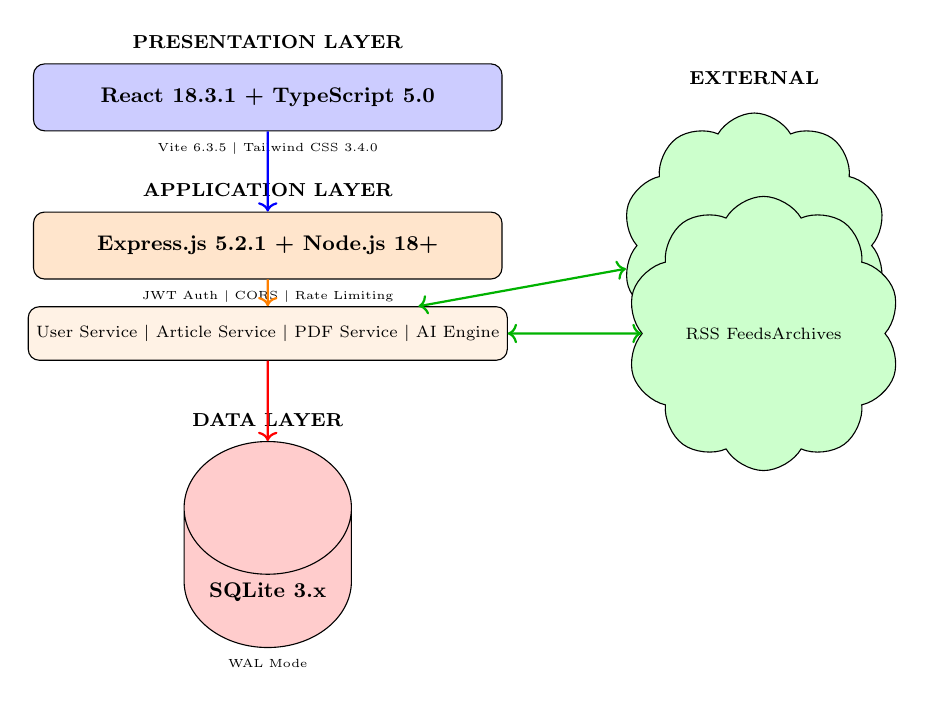
\begin{tikzpicture}[node distance=0.8cm, scale=0.85, every node/.style={transform shape}]

% PRESENTATION LAYER
\node[draw, rectangle, fill=blue!20, rounded corners, minimum width=7cm, minimum height=1cm, font=\small\bfseries] (ui) {React 18.3.1 + TypeScript 5.0};
\node[above=0.1cm of ui, font=\footnotesize\bfseries] {PRESENTATION LAYER};
\node[below=0.05cm of ui, font=\tiny] {Vite 6.3.5 \textbar{} Tailwind CSS 3.4.0};

% APPLICATION LAYER
\node[draw, rectangle, fill=orange!20, rounded corners, minimum width=7cm, minimum height=1cm, below=1.2cm of ui, font=\small\bfseries] (api) {Express.js 5.2.1 + Node.js 18+};
\node[above=0.1cm of api, font=\footnotesize\bfseries] {APPLICATION LAYER};
\node[below=0.05cm of api, font=\tiny] {JWT Auth \textbar{} CORS \textbar{} Rate Limiting};

\node[draw, rectangle, fill=orange!10, rounded corners, minimum width=7cm, minimum height=0.8cm, below=0.4cm of api, font=\scriptsize] (services) {User Service \textbar{} Article Service \textbar{} PDF Service \textbar{} AI Engine};

% DATA LAYER
\node[draw, cylinder, shape border rotate=90, fill=red!20, minimum width=2.5cm, minimum height=1.2cm, below=1.2cm of services, font=\small\bfseries] (db) {SQLite 3.x};
\node[above=0.1cm of db, font=\footnotesize\bfseries] {DATA LAYER};
\node[below=0.05cm of db, font=\tiny] {WAL Mode};

% EXTERNAL SERVICES
\node[draw, cloud, cloud puffs=10, cloud puff arc=120, fill=green!20, minimum width=2.5cm, minimum height=1.5cm, right=2cm of api, font=\scriptsize] (groq) {Groq AI\\Llama 3.3};
\node[draw, cloud, cloud puffs=10, cloud puff arc=120, fill=green!20, minimum width=2.5cm, minimum height=1.5cm, right=2cm of services, font=\scriptsize] (rss) {RSS Feeds\\Archives};
\node[above=0.3cm of groq, font=\footnotesize\bfseries] {EXTERNAL};

% Arrows
\draw[->, thick, blue] (ui) -- (api);
\draw[->, thick, orange] (api) -- (services);
\draw[->, thick, red] (services) -- (db);
\draw[<->, thick, green!70!black] (services) -- (groq);
\draw[<->, thick, green!70!black] (services) -- (rss);

\end{tikzpicture}
\caption{Three-Tier System Architecture with External Service Integration}
\label{fig:architecture}
\end{figure}

\begin{figure}[!t]
\centering
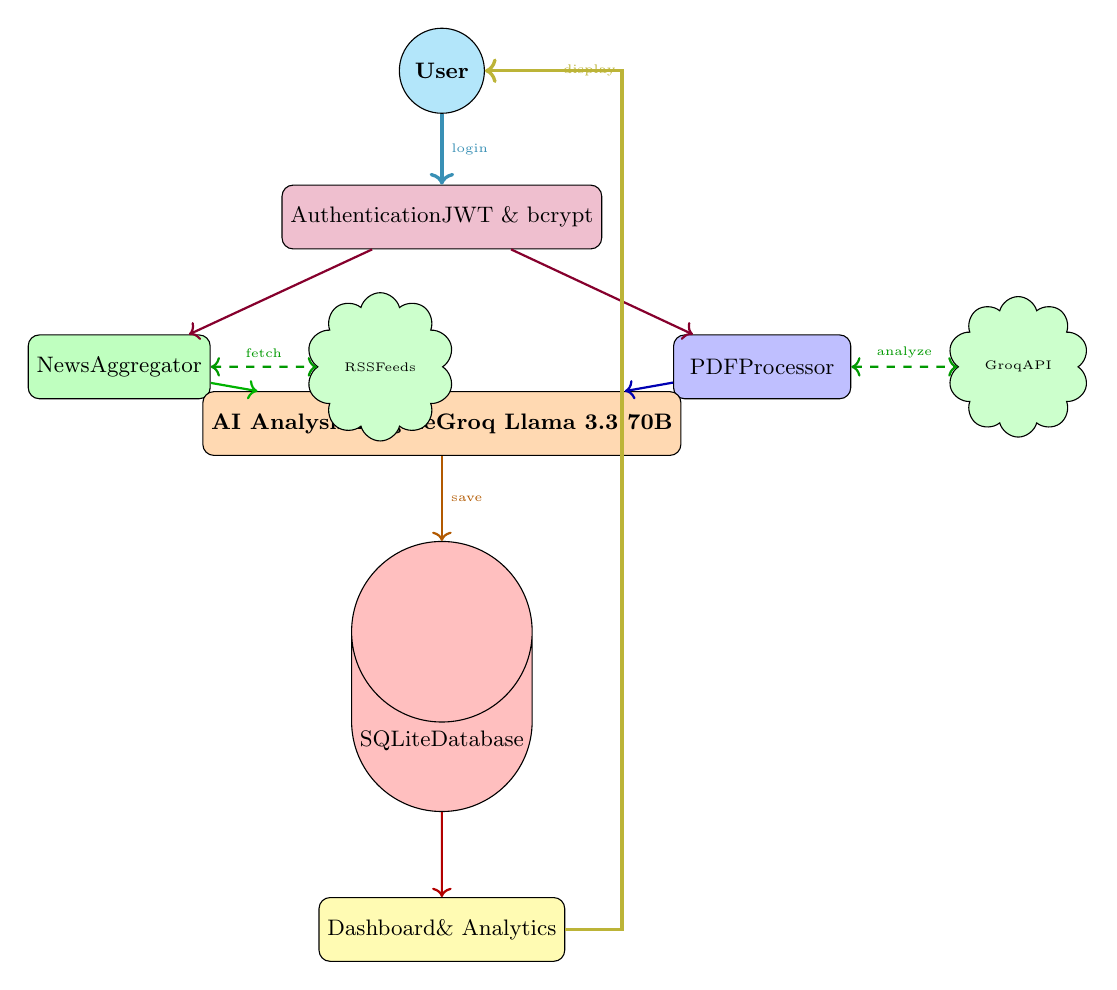
\begin{tikzpicture}[node distance=1cm, scale=0.9, every node/.style={transform shape}]

% User
\node[draw, circle, fill=cyan!30, minimum size=1.2cm, font=\small\bfseries] (user) {User};

% Authentication
\node[draw, rectangle, fill=purple!25, rounded corners, minimum width=3cm, minimum height=0.9cm, below=of user, font=\small] (auth) {Authentication\\JWT \& bcrypt};

% News and PDF processors
\node[draw, rectangle, fill=green!25, rounded corners, minimum width=2.5cm, minimum height=0.9cm, below left=1.2cm and 1cm of auth, font=\small] (news) {News\\Aggregator};
\node[draw, rectangle, fill=blue!25, rounded corners, minimum width=2.5cm, minimum height=0.9cm, below right=1.2cm and 1cm of auth, font=\small] (pdf) {PDF\\Processor};

% AI Engine
\node[draw, rectangle, fill=orange!30, rounded corners, minimum width=3cm, minimum height=0.9cm, below=2cm of auth, font=\small\bfseries] (ai) {AI Analysis Engine\\Groq Llama 3.3 70B};

% Database
\node[draw, cylinder, shape border rotate=90, fill=red!25, minimum width=2.5cm, minimum height=1.2cm, below=1.2cm of ai, font=\small] (db) {SQLite\\Database};

% Dashboard
\node[draw, rectangle, fill=yellow!30, rounded corners, minimum width=3cm, minimum height=0.9cm, below=1.2cm of db, font=\small] (dash) {Dashboard\\\& Analytics};

% External Services
\node[draw, cloud, cloud puffs=10, fill=green!20, minimum width=2cm, minimum height=1.2cm, right=1.5cm of news, font=\tiny] (rss) {RSS\\Feeds};
\node[draw, cloud, cloud puffs=10, fill=green!20, minimum width=2cm, minimum height=1.2cm, right=1.5cm of pdf, font=\tiny] (groq) {Groq\\API};

% Main flow
\draw[->, very thick, cyan!70!black] (user) -- node[right, font=\tiny] {login} (auth);
\draw[->, thick, purple!70!black] (auth) -- (news);
\draw[->, thick, purple!70!black] (auth) -- (pdf);
\draw[->, thick, green!70!black] (news) -- (ai);
\draw[->, thick, blue!70!black] (pdf) -- (ai);
\draw[->, thick, orange!70!black] (ai) -- node[right, font=\tiny] {save} (db);
\draw[->, thick, red!70!black] (db) -- (dash);
\draw[->, very thick, yellow!70!black] (dash.east) -- ++(0.8,0) |- node[near end, right, font=\tiny] {display} (user.east);

% External connections
\draw[<->, thick, dashed, green!60!black] (news) -- node[above, font=\tiny] {fetch} (rss);
\draw[<->, thick, dashed, green!60!black] (pdf) -- node[above, font=\tiny] {analyze} (groq);

\end{tikzpicture}
\caption{System Block Diagram: End-to-End Data Flow from User Input to Analysis Output}
\label{fig:blockdiagram}
\end{figure}

%==========================================================
\section{Results and Evaluation}
%==========================================================

\subsection{Experimental Setup}
System evaluation was conducted using two methodologies: (1)~functional and performance benchmarking on controlled hardware; and (2)~accuracy assessment of AI-generated exam analysis outputs reviewed by the authors and peers familiar with UPSC/SSC syllabi.

\textit{Hardware:} Intel Core i5-12450H (12th Gen, 8 cores, 12 threads), 16\,GB RAM, Windows~11, Node.js~18.16.0, SQLite~3.42.0, 100\,Mbps broadband. \textit{Dataset:} Articles fetched live from five major Indian news sources; 50 PDF documents including UPSC previous-year papers and standard study materials; all 11 language outputs manually inspected.

\subsection{Performance Benchmarks}
Table~\ref{tab:perf} summarizes measured performance. Authentication averaged 145\,ms (including bcrypt hashing); article retrieval 89\,ms for 100 records; statistics endpoint 42\,ms. Under simulated concurrent load, response time remained below 200\,ms with WAL mode enabling parallel reads.

\begin{table}[!t]
\renewcommand{\arraystretch}{1.2}
\caption{System Performance Benchmarks}
\label{tab:perf}
\centering
\small
\begin{tabular}{@{}lcc@{}}
\toprule
\textbf{Metric} & \textbf{Measured} & \textbf{95th Pct.} \\
\midrule
API response time (avg.)     & 150 ms  & 320 ms \\
RSS aggregation (10 sources) & 8.2 s   & ---    \\
Archive mode (30-day range)  & 45 s    & ---    \\
AI analysis per article      & 2.8 s   & 5.1 s  \\
PDF analysis (10 pages)      & 3.2 s   & 6.4 s  \\
PDF text extraction (50 MB)  & 8.5 s   & ---    \\
DB article insert            & 12 ms   & ---    \\
DB query (1{,}000 records)   & 8 ms    & ---    \\
\bottomrule
\end{tabular}
\end{table}

\subsection{Accuracy and Relevance Evaluation}
\textbf{Exam Relevance:} A sample of 100 AI-analyzed articles was reviewed by the authors against UPSC/SSC syllabus categories. Approximately 87\% of outputs contained specific factual details (names, dates, numerical values) directly relevant to examination topics; 11\% were moderately relevant with some generic content; 2\% were considered low relevance.

\textbf{Factual Accuracy:} Cross-verification of extracted facts against source articles across a 50-article sample showed a 96\% match rate; the remaining 4\% contained minor inaccuracies or hallucinated details, primarily in AI-generated potential questions.

\textbf{Multi-Lingual Quality:} All 11 language outputs were inspected for script correctness. Native-script enforcement via LLM prompting achieved 100\% correct Unicode rendering with zero transliteration artifacts. Translation quality was assessed informally for Hindi and Marathi outputs and found to be semantically coherent.

\textbf{PDF Analysis:} Testing on 50 PDF documents (previous-year papers, study notes) showed text extraction accuracy of 97\% for digitally generated PDFs; scanned image-based PDFs are not currently supported (identified as a limitation). AI analysis outputs were reviewed and found to produce relevant key points and examination questions consistent with document content.

\subsection{Comparative Analysis}
Table~\ref{tab:compare} positions the proposed system against commonly used platforms on dimensions relevant to competitive examination preparation.

\begin{table}[!t]
\renewcommand{\arraystretch}{1.2}
\caption{Comparison with Existing Platforms}
\label{tab:compare}
\centering
\small
\begin{tabular}{@{}p{2.0cm}p{1.3cm}p{1.2cm}p{1.6cm}@{}}
\toprule
\textbf{Feature} & \textbf{Proposed} & \textbf{Google News} & \textbf{Inshorts / Dailyhunt} \\
\midrule
Temporal depth      & 10 years    & 7–30 days   & 7–30 days   \\
Exam analysis       & Yes (AI)    & No          & No          \\
PDF processing      & Yes         & No          & No          \\
Indian languages    & 11 (native) & 5 (partial) & 2–5         \\
Relevance scoring   & AI-driven   & Generic     & Generic     \\
Historical archive  & Yes         & No          & No          \\
\bottomrule
\end{tabular}
\end{table}

%==========================================================
\section{Conclusion}
%==========================================================

This paper presented a comprehensive AI-powered system addressing critical challenges in Indian competitive examination preparation through three novel contributions: decade-spanning hybrid news aggregation, exam-focused AI analysis using Groq's Llama~3.3~70B, and a multi-lingual processing pipeline supporting 11 Indian languages with native script enforcement.

System benchmarks demonstrate 150\,ms average API response and 3.2\,s document analysis. Accuracy evaluation on sampled outputs shows 87\% exam relevance and 96\% factual accuracy. The system is functional as a deployed prototype and addresses a clear gap unmet by existing commercial platforms.

Identified limitations include the absence of OCR for scanned PDFs, reliance on third-party LLM APIs introducing latency variability, and the need for broader user evaluation. Future directions include: (1)~expanding to 50+ news sources including regional publications; (2)~integrating spaced-repetition question banks; (3)~developing native iOS/Android applications; (4)~adding Tesseract-based OCR for scanned documents; (5)~implementing study-group collaboration features; and (6)~conducting a formal user study with a representative sample of examination candidates to quantitatively validate usability and learning outcomes.

\begin{thebibliography}{10}

\bibitem{allahyari2017text}
M.~Allahyari, S.~Pouriyeh, M.~Assefi, S.~Safaei, E.~D.~Trippe, J.~B.~Gutierrez, and K.~Kochut, ``Text summarization techniques: A brief survey,'' \textit{Int. J. Adv. Comput. Sci. Appl.}, vol.~8, no.~10, 2017.

\bibitem{alomari2022deep}
A.~Alomari, N.~Idris, A.~Q.~M.~Sabri, and I.~Alsmadi, ``Deep reinforcement and transfer learning for abstractive text summarization: A review,'' \textit{Comput. Speech Lang.}, vol.~71, p.~101276, 2022.

\bibitem{cao2022hallucinated}
M.~Cao, Y.~Dong, and J.~Cheung, ``Hallucinated but factual! Inspecting the factuality of hallucinations in abstractive summarization,'' in \textit{Proc. 60th Annu. Meeting Assoc. Comput. Linguistics (ACL)}, 2022, pp.~3340--3354.

\bibitem{aharoni2022mface}
R.~Aharoni, S.~Narayan, J.~Maynez, J.~Herzig, E.~Clark, and M.~Lapata, ``mFACE: Multilingual summarization with factual consistency evaluation,'' \textit{arXiv preprint arXiv:2212.10622}, 2022.

\bibitem{amato2017semantic}
F.~Amato, A.~D'Acierno, F.~Colace, V.~Moscato, A.~Penta, and A.~Picariello, ``Semantic summarization of news from heterogeneous sources,'' in \textit{Proc. IEEE Int. Conf. Semantic Computing (ICSC)}, 2017, pp.~174--177.

\bibitem{alias2021unsupervised}
S.~Alias, ``Unsupervised text feature extraction for academic chatbot using constrained FP-growth,'' \textit{ASM Sci. J.}, vol.~14, pp.~1--11, 2021.

\bibitem{alam2003structured}
H.~Alam, A.~Kumar, M.~Nakamura, F.~Rahman, Y.~Tarnikova, and C.~Wilcox, ``Structured and unstructured document summarization: Design of a commercial summarizer using lexical chains,'' in \textit{Proc. 7th Int. Conf. Document Anal. Recognition (ICDAR)}, vol.~1, 2003, pp.~1147--1152.

\bibitem{bao2020unilmv2}
H.~Bao \textit{et al.}, ``UniLMv2: Pseudo-masked language models for unified language model pre-training,'' in \textit{Proc. 37th Int. Conf. Mach. Learn. (ICML)}, vol.~119, 2020, pp.~642--652.

\bibitem{brazinskas2020fewshot}
A.~Brazinskas, M.~Lapata, and I.~Titov, ``Few-shot learning for opinion summarization,'' in \textit{Proc. Conf. Empirical Methods Natural Language Process. (EMNLP)}, 2020, pp.~4119--4135.

\bibitem{cao2020factual}
M.~Cao, Y.~Dong, J.~Wu, and J.~C.~K.~Cheung, ``Factual error correction for abstractive summarization models,'' in \textit{Proc. Conf. Empirical Methods Natural Language Process. (EMNLP)}, 2020, pp.~6251--6258.

\end{thebibliography}

\end{document}